\documentclass[]{article}
\usepackage{lmodern}
\usepackage{amssymb,amsmath}
\usepackage{ifxetex,ifluatex}
\usepackage{fixltx2e} % provides \textsubscript
\ifnum 0\ifxetex 1\fi\ifluatex 1\fi=0 % if pdftex
  \usepackage[T1]{fontenc}
  \usepackage[utf8]{inputenc}
\else % if luatex or xelatex
  \ifxetex
    \usepackage{mathspec}
  \else
    \usepackage{fontspec}
  \fi
  \defaultfontfeatures{Ligatures=TeX,Scale=MatchLowercase}
\fi
% use upquote if available, for straight quotes in verbatim environments
\IfFileExists{upquote.sty}{\usepackage{upquote}}{}
% use microtype if available
\IfFileExists{microtype.sty}{%
\usepackage{microtype}
\UseMicrotypeSet[protrusion]{basicmath} % disable protrusion for tt fonts
}{}
\usepackage[margin=0.25in]{geometry}
\usepackage{hyperref}
\hypersetup{unicode=true,
            pdftitle={STAT565\_Lab},
            pdfauthor={Shen Qu},
            pdfborder={0 0 0},
            breaklinks=true}
\urlstyle{same}  % don't use monospace font for urls
\usepackage{color}
\usepackage{fancyvrb}
\newcommand{\VerbBar}{|}
\newcommand{\VERB}{\Verb[commandchars=\\\{\}]}
\DefineVerbatimEnvironment{Highlighting}{Verbatim}{commandchars=\\\{\}}
% Add ',fontsize=\small' for more characters per line
\usepackage{framed}
\definecolor{shadecolor}{RGB}{248,248,248}
\newenvironment{Shaded}{\begin{snugshade}}{\end{snugshade}}
\newcommand{\AlertTok}[1]{\textcolor[rgb]{0.94,0.16,0.16}{#1}}
\newcommand{\AnnotationTok}[1]{\textcolor[rgb]{0.56,0.35,0.01}{\textbf{\textit{#1}}}}
\newcommand{\AttributeTok}[1]{\textcolor[rgb]{0.77,0.63,0.00}{#1}}
\newcommand{\BaseNTok}[1]{\textcolor[rgb]{0.00,0.00,0.81}{#1}}
\newcommand{\BuiltInTok}[1]{#1}
\newcommand{\CharTok}[1]{\textcolor[rgb]{0.31,0.60,0.02}{#1}}
\newcommand{\CommentTok}[1]{\textcolor[rgb]{0.56,0.35,0.01}{\textit{#1}}}
\newcommand{\CommentVarTok}[1]{\textcolor[rgb]{0.56,0.35,0.01}{\textbf{\textit{#1}}}}
\newcommand{\ConstantTok}[1]{\textcolor[rgb]{0.00,0.00,0.00}{#1}}
\newcommand{\ControlFlowTok}[1]{\textcolor[rgb]{0.13,0.29,0.53}{\textbf{#1}}}
\newcommand{\DataTypeTok}[1]{\textcolor[rgb]{0.13,0.29,0.53}{#1}}
\newcommand{\DecValTok}[1]{\textcolor[rgb]{0.00,0.00,0.81}{#1}}
\newcommand{\DocumentationTok}[1]{\textcolor[rgb]{0.56,0.35,0.01}{\textbf{\textit{#1}}}}
\newcommand{\ErrorTok}[1]{\textcolor[rgb]{0.64,0.00,0.00}{\textbf{#1}}}
\newcommand{\ExtensionTok}[1]{#1}
\newcommand{\FloatTok}[1]{\textcolor[rgb]{0.00,0.00,0.81}{#1}}
\newcommand{\FunctionTok}[1]{\textcolor[rgb]{0.00,0.00,0.00}{#1}}
\newcommand{\ImportTok}[1]{#1}
\newcommand{\InformationTok}[1]{\textcolor[rgb]{0.56,0.35,0.01}{\textbf{\textit{#1}}}}
\newcommand{\KeywordTok}[1]{\textcolor[rgb]{0.13,0.29,0.53}{\textbf{#1}}}
\newcommand{\NormalTok}[1]{#1}
\newcommand{\OperatorTok}[1]{\textcolor[rgb]{0.81,0.36,0.00}{\textbf{#1}}}
\newcommand{\OtherTok}[1]{\textcolor[rgb]{0.56,0.35,0.01}{#1}}
\newcommand{\PreprocessorTok}[1]{\textcolor[rgb]{0.56,0.35,0.01}{\textit{#1}}}
\newcommand{\RegionMarkerTok}[1]{#1}
\newcommand{\SpecialCharTok}[1]{\textcolor[rgb]{0.00,0.00,0.00}{#1}}
\newcommand{\SpecialStringTok}[1]{\textcolor[rgb]{0.31,0.60,0.02}{#1}}
\newcommand{\StringTok}[1]{\textcolor[rgb]{0.31,0.60,0.02}{#1}}
\newcommand{\VariableTok}[1]{\textcolor[rgb]{0.00,0.00,0.00}{#1}}
\newcommand{\VerbatimStringTok}[1]{\textcolor[rgb]{0.31,0.60,0.02}{#1}}
\newcommand{\WarningTok}[1]{\textcolor[rgb]{0.56,0.35,0.01}{\textbf{\textit{#1}}}}
\usepackage{longtable,booktabs}
\usepackage{graphicx,grffile}
\makeatletter
\def\maxwidth{\ifdim\Gin@nat@width>\linewidth\linewidth\else\Gin@nat@width\fi}
\def\maxheight{\ifdim\Gin@nat@height>\textheight\textheight\else\Gin@nat@height\fi}
\makeatother
% Scale images if necessary, so that they will not overflow the page
% margins by default, and it is still possible to overwrite the defaults
% using explicit options in \includegraphics[width, height, ...]{}
\setkeys{Gin}{width=\maxwidth,height=\maxheight,keepaspectratio}
\IfFileExists{parskip.sty}{%
\usepackage{parskip}
}{% else
\setlength{\parindent}{0pt}
\setlength{\parskip}{6pt plus 2pt minus 1pt}
}
\setlength{\emergencystretch}{3em}  % prevent overfull lines
\providecommand{\tightlist}{%
  \setlength{\itemsep}{0pt}\setlength{\parskip}{0pt}}
\setcounter{secnumdepth}{0}
% Redefines (sub)paragraphs to behave more like sections
\ifx\paragraph\undefined\else
\let\oldparagraph\paragraph
\renewcommand{\paragraph}[1]{\oldparagraph{#1}\mbox{}}
\fi
\ifx\subparagraph\undefined\else
\let\oldsubparagraph\subparagraph
\renewcommand{\subparagraph}[1]{\oldsubparagraph{#1}\mbox{}}
\fi

%%% Use protect on footnotes to avoid problems with footnotes in titles
\let\rmarkdownfootnote\footnote%
\def\footnote{\protect\rmarkdownfootnote}

%%% Change title format to be more compact
\usepackage{titling}

% Create subtitle command for use in maketitle
\newcommand{\subtitle}[1]{
  \posttitle{
    \begin{center}\large#1\end{center}
    }
}

\setlength{\droptitle}{-2em}

  \title{STAT565\_Lab}
    \pretitle{\vspace{\droptitle}\centering\huge}
  \posttitle{\par}
    \author{Shen Qu}
    \preauthor{\centering\large\emph}
  \postauthor{\par}
      \predate{\centering\large\emph}
  \postdate{\par}
    \date{March 12, 2019}


\begin{document}
\maketitle

(a).
\textcolor[rgb]{0.5,0.5,0.5}{Plot the data and report the plot here (A plot with data and means of treatment combinations). Do not report code here. Describe the observed relationship between two factors.}

\begin{verbatim}
## Observations: 40
## Variables: 5
## $ Source <chr> "Beef", "Beef", "Beef", "Beef", "Beef", "Beef", "Beef",...
## $ Amount <chr> "Low", "Low", "Low", "Low", "Low", "Low", "Low", "Low",...
## $ Gain   <dbl> 90, 76, 90, 64, 86, 51, 72, 90, 95, 78, 73, 102, 118, 1...
## $ Trt1   <fct> Beef, Beef, Beef, Beef, Beef, Beef, Beef, Beef, Beef, B...
## $ Trt2   <fct> Low, Low, Low, Low, Low, Low, Low, Low, Low, Low, High,...
\end{verbatim}

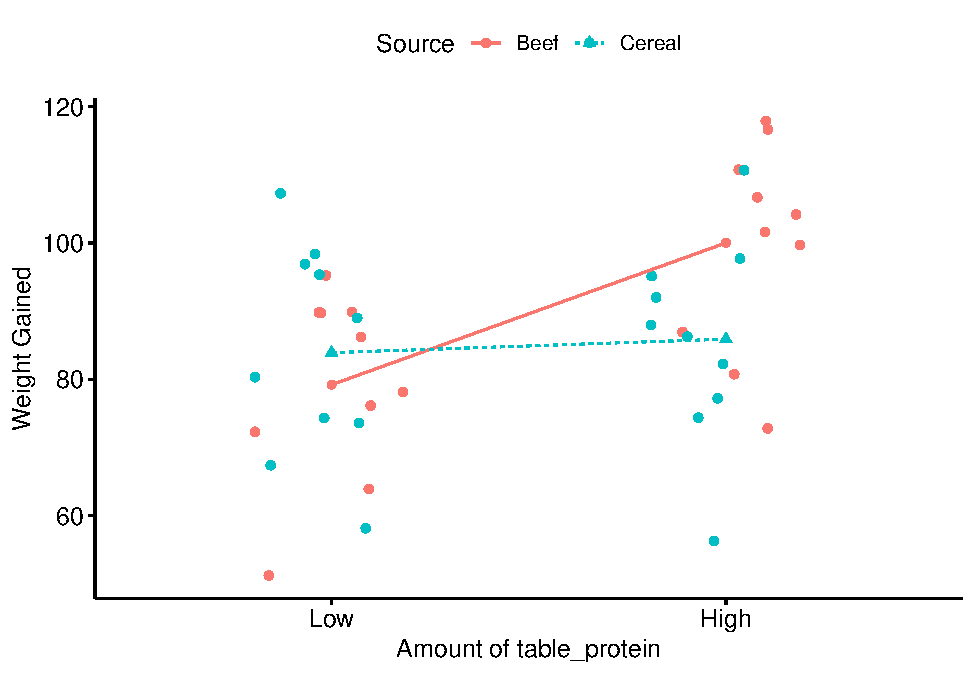
\includegraphics[width=0.5\linewidth]{lab_stat565_files/figure-latex/unnamed-chunk-3-1}

(b).
\textcolor[rgb]{0.5,0.5,0.5}{Obtain the numerical summary for each treatment combination and factor levels separately. Report them here in a tabular form.}

\begin{longtable}[]{@{}cccccccccc@{}}
\toprule
\begin{minipage}[b]{0.09\columnwidth}\centering
Source\strut
\end{minipage} & \begin{minipage}[b]{0.06\columnwidth}\centering
min\strut
\end{minipage} & \begin{minipage}[b]{0.07\columnwidth}\centering
Q1\strut
\end{minipage} & \begin{minipage}[b]{0.09\columnwidth}\centering
median\strut
\end{minipage} & \begin{minipage}[b]{0.08\columnwidth}\centering
Q3\strut
\end{minipage} & \begin{minipage}[b]{0.06\columnwidth}\centering
max\strut
\end{minipage} & \begin{minipage}[b]{0.07\columnwidth}\centering
mean\strut
\end{minipage} & \begin{minipage}[b]{0.08\columnwidth}\centering
sd\strut
\end{minipage} & \begin{minipage}[b]{0.05\columnwidth}\centering
n\strut
\end{minipage} & \begin{minipage}[b]{0.10\columnwidth}\centering
missing\strut
\end{minipage}\tabularnewline
\midrule
\endhead
\begin{minipage}[t]{0.09\columnwidth}\centering
Beef\strut
\end{minipage} & \begin{minipage}[t]{0.06\columnwidth}\centering
51\strut
\end{minipage} & \begin{minipage}[t]{0.07\columnwidth}\centering
77.5\strut
\end{minipage} & \begin{minipage}[t]{0.09\columnwidth}\centering
90\strut
\end{minipage} & \begin{minipage}[t]{0.08\columnwidth}\centering
102.5\strut
\end{minipage} & \begin{minipage}[t]{0.06\columnwidth}\centering
118\strut
\end{minipage} & \begin{minipage}[t]{0.07\columnwidth}\centering
89.6\strut
\end{minipage} & \begin{minipage}[t]{0.08\columnwidth}\centering
17.71\strut
\end{minipage} & \begin{minipage}[t]{0.05\columnwidth}\centering
20\strut
\end{minipage} & \begin{minipage}[t]{0.10\columnwidth}\centering
0\strut
\end{minipage}\tabularnewline
\begin{minipage}[t]{0.09\columnwidth}\centering
Cereal\strut
\end{minipage} & \begin{minipage}[t]{0.06\columnwidth}\centering
56\strut
\end{minipage} & \begin{minipage}[t]{0.07\columnwidth}\centering
74\strut
\end{minipage} & \begin{minipage}[t]{0.09\columnwidth}\centering
87\strut
\end{minipage} & \begin{minipage}[t]{0.08\columnwidth}\centering
95.5\strut
\end{minipage} & \begin{minipage}[t]{0.06\columnwidth}\centering
111\strut
\end{minipage} & \begin{minipage}[t]{0.07\columnwidth}\centering
84.9\strut
\end{minipage} & \begin{minipage}[t]{0.08\columnwidth}\centering
14.99\strut
\end{minipage} & \begin{minipage}[t]{0.05\columnwidth}\centering
20\strut
\end{minipage} & \begin{minipage}[t]{0.10\columnwidth}\centering
0\strut
\end{minipage}\tabularnewline
\bottomrule
\end{longtable}

\begin{longtable}[]{@{}cccccccccc@{}}
\toprule
\begin{minipage}[b]{0.13\columnwidth}\centering
Amount\strut
\end{minipage} & \begin{minipage}[b]{0.05\columnwidth}\centering
min\strut
\end{minipage} & \begin{minipage}[b]{0.07\columnwidth}\centering
Q1\strut
\end{minipage} & \begin{minipage}[b]{0.08\columnwidth}\centering
median\strut
\end{minipage} & \begin{minipage}[b]{0.07\columnwidth}\centering
Q3\strut
\end{minipage} & \begin{minipage}[b]{0.05\columnwidth}\centering
max\strut
\end{minipage} & \begin{minipage}[b]{0.07\columnwidth}\centering
mean\strut
\end{minipage} & \begin{minipage}[b]{0.07\columnwidth}\centering
sd\strut
\end{minipage} & \begin{minipage}[b]{0.04\columnwidth}\centering
n\strut
\end{minipage} & \begin{minipage}[b]{0.09\columnwidth}\centering
missing\strut
\end{minipage}\tabularnewline
\midrule
\endhead
\begin{minipage}[t]{0.13\columnwidth}\centering
Beef.High\strut
\end{minipage} & \begin{minipage}[t]{0.05\columnwidth}\centering
73\strut
\end{minipage} & \begin{minipage}[t]{0.07\columnwidth}\centering
90.25\strut
\end{minipage} & \begin{minipage}[t]{0.08\columnwidth}\centering
103\strut
\end{minipage} & \begin{minipage}[t]{0.07\columnwidth}\centering
110\strut
\end{minipage} & \begin{minipage}[t]{0.05\columnwidth}\centering
118\strut
\end{minipage} & \begin{minipage}[t]{0.07\columnwidth}\centering
100\strut
\end{minipage} & \begin{minipage}[t]{0.07\columnwidth}\centering
15.14\strut
\end{minipage} & \begin{minipage}[t]{0.04\columnwidth}\centering
10\strut
\end{minipage} & \begin{minipage}[t]{0.09\columnwidth}\centering
0\strut
\end{minipage}\tabularnewline
\begin{minipage}[t]{0.13\columnwidth}\centering
Cereal.High\strut
\end{minipage} & \begin{minipage}[t]{0.05\columnwidth}\centering
56\strut
\end{minipage} & \begin{minipage}[t]{0.07\columnwidth}\centering
78.25\strut
\end{minipage} & \begin{minipage}[t]{0.08\columnwidth}\centering
87\strut
\end{minipage} & \begin{minipage}[t]{0.07\columnwidth}\centering
94.25\strut
\end{minipage} & \begin{minipage}[t]{0.05\columnwidth}\centering
111\strut
\end{minipage} & \begin{minipage}[t]{0.07\columnwidth}\centering
85.9\strut
\end{minipage} & \begin{minipage}[t]{0.07\columnwidth}\centering
15.02\strut
\end{minipage} & \begin{minipage}[t]{0.04\columnwidth}\centering
10\strut
\end{minipage} & \begin{minipage}[t]{0.09\columnwidth}\centering
0\strut
\end{minipage}\tabularnewline
\begin{minipage}[t]{0.13\columnwidth}\centering
Beef.Low\strut
\end{minipage} & \begin{minipage}[t]{0.05\columnwidth}\centering
51\strut
\end{minipage} & \begin{minipage}[t]{0.07\columnwidth}\centering
73\strut
\end{minipage} & \begin{minipage}[t]{0.08\columnwidth}\centering
82\strut
\end{minipage} & \begin{minipage}[t]{0.07\columnwidth}\centering
90\strut
\end{minipage} & \begin{minipage}[t]{0.05\columnwidth}\centering
95\strut
\end{minipage} & \begin{minipage}[t]{0.07\columnwidth}\centering
79.2\strut
\end{minipage} & \begin{minipage}[t]{0.07\columnwidth}\centering
13.89\strut
\end{minipage} & \begin{minipage}[t]{0.04\columnwidth}\centering
10\strut
\end{minipage} & \begin{minipage}[t]{0.09\columnwidth}\centering
0\strut
\end{minipage}\tabularnewline
\begin{minipage}[t]{0.13\columnwidth}\centering
Cereal.Low\strut
\end{minipage} & \begin{minipage}[t]{0.05\columnwidth}\centering
58\strut
\end{minipage} & \begin{minipage}[t]{0.07\columnwidth}\centering
74\strut
\end{minipage} & \begin{minipage}[t]{0.08\columnwidth}\centering
84.5\strut
\end{minipage} & \begin{minipage}[t]{0.07\columnwidth}\centering
96.5\strut
\end{minipage} & \begin{minipage}[t]{0.05\columnwidth}\centering
107\strut
\end{minipage} & \begin{minipage}[t]{0.07\columnwidth}\centering
83.9\strut
\end{minipage} & \begin{minipage}[t]{0.07\columnwidth}\centering
15.71\strut
\end{minipage} & \begin{minipage}[t]{0.04\columnwidth}\centering
10\strut
\end{minipage} & \begin{minipage}[t]{0.09\columnwidth}\centering
0\strut
\end{minipage}\tabularnewline
\begin{minipage}[t]{0.13\columnwidth}\centering
High\strut
\end{minipage} & \begin{minipage}[t]{0.05\columnwidth}\centering
56\strut
\end{minipage} & \begin{minipage}[t]{0.07\columnwidth}\centering
81.75\strut
\end{minipage} & \begin{minipage}[t]{0.08\columnwidth}\centering
93.5\strut
\end{minipage} & \begin{minipage}[t]{0.07\columnwidth}\centering
104.8\strut
\end{minipage} & \begin{minipage}[t]{0.05\columnwidth}\centering
118\strut
\end{minipage} & \begin{minipage}[t]{0.07\columnwidth}\centering
92.95\strut
\end{minipage} & \begin{minipage}[t]{0.07\columnwidth}\centering
16.36\strut
\end{minipage} & \begin{minipage}[t]{0.04\columnwidth}\centering
20\strut
\end{minipage} & \begin{minipage}[t]{0.09\columnwidth}\centering
0\strut
\end{minipage}\tabularnewline
\begin{minipage}[t]{0.13\columnwidth}\centering
Low\strut
\end{minipage} & \begin{minipage}[t]{0.05\columnwidth}\centering
51\strut
\end{minipage} & \begin{minipage}[t]{0.07\columnwidth}\centering
73.5\strut
\end{minipage} & \begin{minipage}[t]{0.08\columnwidth}\centering
83\strut
\end{minipage} & \begin{minipage}[t]{0.07\columnwidth}\centering
91.25\strut
\end{minipage} & \begin{minipage}[t]{0.05\columnwidth}\centering
107\strut
\end{minipage} & \begin{minipage}[t]{0.07\columnwidth}\centering
81.55\strut
\end{minipage} & \begin{minipage}[t]{0.07\columnwidth}\centering
14.63\strut
\end{minipage} & \begin{minipage}[t]{0.04\columnwidth}\centering
20\strut
\end{minipage} & \begin{minipage}[t]{0.09\columnwidth}\centering
0\strut
\end{minipage}\tabularnewline
\bottomrule
\end{longtable}

(c).
\textcolor[rgb]{0.5,0.5,0.5}{Fit the two-factor factorial model and report the complete ANOVA table here. Do not report code here. The complete ANOVA table should have a row for each of the following: main effects of each treatment, two-factor interaction effects, error and total.}

\begin{longtable}[]{@{}crrrrr@{}}
\toprule
\begin{minipage}[b]{0.19\columnwidth}\centering
~\strut
\end{minipage} & \begin{minipage}[b]{0.06\columnwidth}\raggedleft
Df\strut
\end{minipage} & \begin{minipage}[b]{0.10\columnwidth}\raggedleft
Sum Sq\strut
\end{minipage} & \begin{minipage}[b]{0.12\columnwidth}\raggedleft
Mean Sq\strut
\end{minipage} & \begin{minipage}[b]{0.12\columnwidth}\raggedleft
F value\strut
\end{minipage} & \begin{minipage}[b]{0.12\columnwidth}\raggedleft
Pr(\textgreater{}F)\strut
\end{minipage}\tabularnewline
\midrule
\endhead
\begin{minipage}[t]{0.19\columnwidth}\centering
\textbf{Trt1}\strut
\end{minipage} & \begin{minipage}[t]{0.06\columnwidth}\raggedleft
1\strut
\end{minipage} & \begin{minipage}[t]{0.10\columnwidth}\raggedleft
220.9\strut
\end{minipage} & \begin{minipage}[t]{0.12\columnwidth}\raggedleft
220.9\strut
\end{minipage} & \begin{minipage}[t]{0.12\columnwidth}\raggedleft
0.9879\strut
\end{minipage} & \begin{minipage}[t]{0.12\columnwidth}\raggedleft
0.3269\strut
\end{minipage}\tabularnewline
\begin{minipage}[t]{0.19\columnwidth}\centering
\textbf{Trt2}\strut
\end{minipage} & \begin{minipage}[t]{0.06\columnwidth}\raggedleft
1\strut
\end{minipage} & \begin{minipage}[t]{0.10\columnwidth}\raggedleft
1300\strut
\end{minipage} & \begin{minipage}[t]{0.12\columnwidth}\raggedleft
1300\strut
\end{minipage} & \begin{minipage}[t]{0.12\columnwidth}\raggedleft
5.812\strut
\end{minipage} & \begin{minipage}[t]{0.12\columnwidth}\raggedleft
0.02114\strut
\end{minipage}\tabularnewline
\begin{minipage}[t]{0.19\columnwidth}\centering
\textbf{Trt1:Trt2}\strut
\end{minipage} & \begin{minipage}[t]{0.06\columnwidth}\raggedleft
1\strut
\end{minipage} & \begin{minipage}[t]{0.10\columnwidth}\raggedleft
883.6\strut
\end{minipage} & \begin{minipage}[t]{0.12\columnwidth}\raggedleft
883.6\strut
\end{minipage} & \begin{minipage}[t]{0.12\columnwidth}\raggedleft
3.952\strut
\end{minipage} & \begin{minipage}[t]{0.12\columnwidth}\raggedleft
0.05447\strut
\end{minipage}\tabularnewline
\begin{minipage}[t]{0.19\columnwidth}\centering
\textbf{Residuals}\strut
\end{minipage} & \begin{minipage}[t]{0.06\columnwidth}\raggedleft
36\strut
\end{minipage} & \begin{minipage}[t]{0.10\columnwidth}\raggedleft
8049\strut
\end{minipage} & \begin{minipage}[t]{0.12\columnwidth}\raggedleft
223.6\strut
\end{minipage} & \begin{minipage}[t]{0.12\columnwidth}\raggedleft
NA\strut
\end{minipage} & \begin{minipage}[t]{0.12\columnwidth}\raggedleft
NA\strut
\end{minipage}\tabularnewline
\begin{minipage}[t]{0.19\columnwidth}\centering
\textbf{Total}\strut
\end{minipage} & \begin{minipage}[t]{0.06\columnwidth}\raggedleft
39\strut
\end{minipage} & \begin{minipage}[t]{0.10\columnwidth}\raggedleft
10453.5\strut
\end{minipage} & \begin{minipage}[t]{0.12\columnwidth}\raggedleft
268.0385\strut
\end{minipage} & \begin{minipage}[t]{0.12\columnwidth}\raggedleft
NA\strut
\end{minipage} & \begin{minipage}[t]{0.12\columnwidth}\raggedleft
NA\strut
\end{minipage}\tabularnewline
\bottomrule
\end{longtable}

(d).
\textcolor[rgb]{0.5,0.5,0.5}{Based on the ANOVA table write your conclusion appropriately. Perform all the necessary tests and report the conclusion along with the p-value.}

The line plot shows that not all lines are parallel. Difference in Gain
between Trt1 is not same for different Trt2. There could be an
interaction effect.

According to ANOVA table, there is a significant interaction effect from
Trt1 and Trt2 on the Gain around 5\% significance level
(P-value=0.05447). That means, effect of method and effect of Trt1 and
Trt2 on Gain is not independent. Therefore, examie the simple effects.

The table shows the simple comparisons of Trt1 Least Squares Means by
Trt2 and Trt2 Least Squares Means by Trt1. Both Tukey and Scheffe
methods indicate the difference in Gain between high-protein and
low-protein is significant when Beef is applies (P-calue=0.01827,0.0338,
respectively). The confidence intervals also support this results.

\begin{longtable}[]{@{}cccccllc@{}}
\toprule
\begin{minipage}[b]{0.24\columnwidth}\centering
~ ~\strut
\end{minipage} & \begin{minipage}[b]{0.07\columnwidth}\centering
diff\strut
\end{minipage} & \begin{minipage}[b]{0.07\columnwidth}\centering
lwr\strut
\end{minipage} & \begin{minipage}[b]{0.07\columnwidth}\centering
Tukey upr\strut
\end{minipage} & \begin{minipage}[b]{0.10\columnwidth}\centering
p adj\strut
\end{minipage} & \begin{minipage}[b]{0.07\columnwidth}\raggedright
lwr.ci\strut
\end{minipage} & \begin{minipage}[b]{0.07\columnwidth}\raggedright
Scheffe upr.ci\strut
\end{minipage} & \begin{minipage}[b]{0.08\columnwidth}\centering
pval\strut
\end{minipage}\tabularnewline
\midrule
\endhead
\begin{minipage}[t]{0.24\columnwidth}\centering
\textbf{Cereal:High-Beef:High}\strut
\end{minipage} & \begin{minipage}[t]{0.07\columnwidth}\centering
-14.1\strut
\end{minipage} & \begin{minipage}[t]{0.07\columnwidth}\centering
-32.11\strut
\end{minipage} & \begin{minipage}[t]{0.07\columnwidth}\centering
3.91\strut
\end{minipage} & \begin{minipage}[t]{0.10\columnwidth}\centering
0.1698\strut
\end{minipage} & \begin{minipage}[t]{0.07\columnwidth}\raggedright
-33.71\strut
\end{minipage} & \begin{minipage}[t]{0.07\columnwidth}\raggedright
5.509\strut
\end{minipage} & \begin{minipage}[t]{0.08\columnwidth}\centering
0.2358\strut
\end{minipage}\tabularnewline
\begin{minipage}[t]{0.24\columnwidth}\centering
\textbf{Beef:Low-Beef:High}\strut
\end{minipage} & \begin{minipage}[t]{0.07\columnwidth}\centering
-20.8\strut
\end{minipage} & \begin{minipage}[t]{0.07\columnwidth}\centering
-38.81\strut
\end{minipage} & \begin{minipage}[t]{0.07\columnwidth}\centering
-2.79\strut
\end{minipage} & \begin{minipage}[t]{0.10\columnwidth}\centering
\textbf{0.01827}\strut
\end{minipage} & \begin{minipage}[t]{0.07\columnwidth}\raggedright
-40.41\strut
\end{minipage} & \begin{minipage}[t]{0.07\columnwidth}\raggedright
-1.191\strut
\end{minipage} & \begin{minipage}[t]{0.08\columnwidth}\centering
\textbf{0.0338}\strut
\end{minipage}\tabularnewline
\begin{minipage}[t]{0.24\columnwidth}\centering
\textbf{Cereal:Low-Beef:High}\strut
\end{minipage} & \begin{minipage}[t]{0.07\columnwidth}\centering
-16.1\strut
\end{minipage} & \begin{minipage}[t]{0.07\columnwidth}\centering
-34.11\strut
\end{minipage} & \begin{minipage}[t]{0.07\columnwidth}\centering
1.91\strut
\end{minipage} & \begin{minipage}[t]{0.10\columnwidth}\centering
0.0937\strut
\end{minipage} & \begin{minipage}[t]{0.07\columnwidth}\raggedright
-35.71\strut
\end{minipage} & \begin{minipage}[t]{0.07\columnwidth}\raggedright
3.509\strut
\end{minipage} & \begin{minipage}[t]{0.08\columnwidth}\centering
0.1418\strut
\end{minipage}\tabularnewline
\begin{minipage}[t]{0.24\columnwidth}\centering
\textbf{Beef:Low-Cereal:High}\strut
\end{minipage} & \begin{minipage}[t]{0.07\columnwidth}\centering
-6.7\strut
\end{minipage} & \begin{minipage}[t]{0.07\columnwidth}\centering
-24.71\strut
\end{minipage} & \begin{minipage}[t]{0.07\columnwidth}\centering
11.31\strut
\end{minipage} & \begin{minipage}[t]{0.10\columnwidth}\centering
0.7493\strut
\end{minipage} & \begin{minipage}[t]{0.07\columnwidth}\raggedright
-26.31\strut
\end{minipage} & \begin{minipage}[t]{0.07\columnwidth}\raggedright
12.91\strut
\end{minipage} & \begin{minipage}[t]{0.08\columnwidth}\centering
0.8004\strut
\end{minipage}\tabularnewline
\begin{minipage}[t]{0.24\columnwidth}\centering
\textbf{Cereal:Low-Cereal:High}\strut
\end{minipage} & \begin{minipage}[t]{0.07\columnwidth}\centering
-2\strut
\end{minipage} & \begin{minipage}[t]{0.07\columnwidth}\centering
-20.01\strut
\end{minipage} & \begin{minipage}[t]{0.07\columnwidth}\centering
16.01\strut
\end{minipage} & \begin{minipage}[t]{0.10\columnwidth}\centering
0.9905\strut
\end{minipage} & \begin{minipage}[t]{0.07\columnwidth}\raggedright
-21.61\strut
\end{minipage} & \begin{minipage}[t]{0.07\columnwidth}\raggedright
17.61\strut
\end{minipage} & \begin{minipage}[t]{0.08\columnwidth}\centering
0.9929\strut
\end{minipage}\tabularnewline
\begin{minipage}[t]{0.24\columnwidth}\centering
\textbf{Cereal:Low-Beef:Low}\strut
\end{minipage} & \begin{minipage}[t]{0.07\columnwidth}\centering
4.7\strut
\end{minipage} & \begin{minipage}[t]{0.07\columnwidth}\centering
-13.31\strut
\end{minipage} & \begin{minipage}[t]{0.07\columnwidth}\centering
22.71\strut
\end{minipage} & \begin{minipage}[t]{0.10\columnwidth}\centering
0.8953\strut
\end{minipage} & \begin{minipage}[t]{0.07\columnwidth}\raggedright
-14.91\strut
\end{minipage} & \begin{minipage}[t]{0.07\columnwidth}\raggedright
24.31\strut
\end{minipage} & \begin{minipage}[t]{0.08\columnwidth}\centering
0.9195\strut
\end{minipage}\tabularnewline
\bottomrule
\end{longtable}

(e).
\textcolor[rgb]{0.5,0.5,0.5}{Provide the plots of residuals here. Do not report code here.}

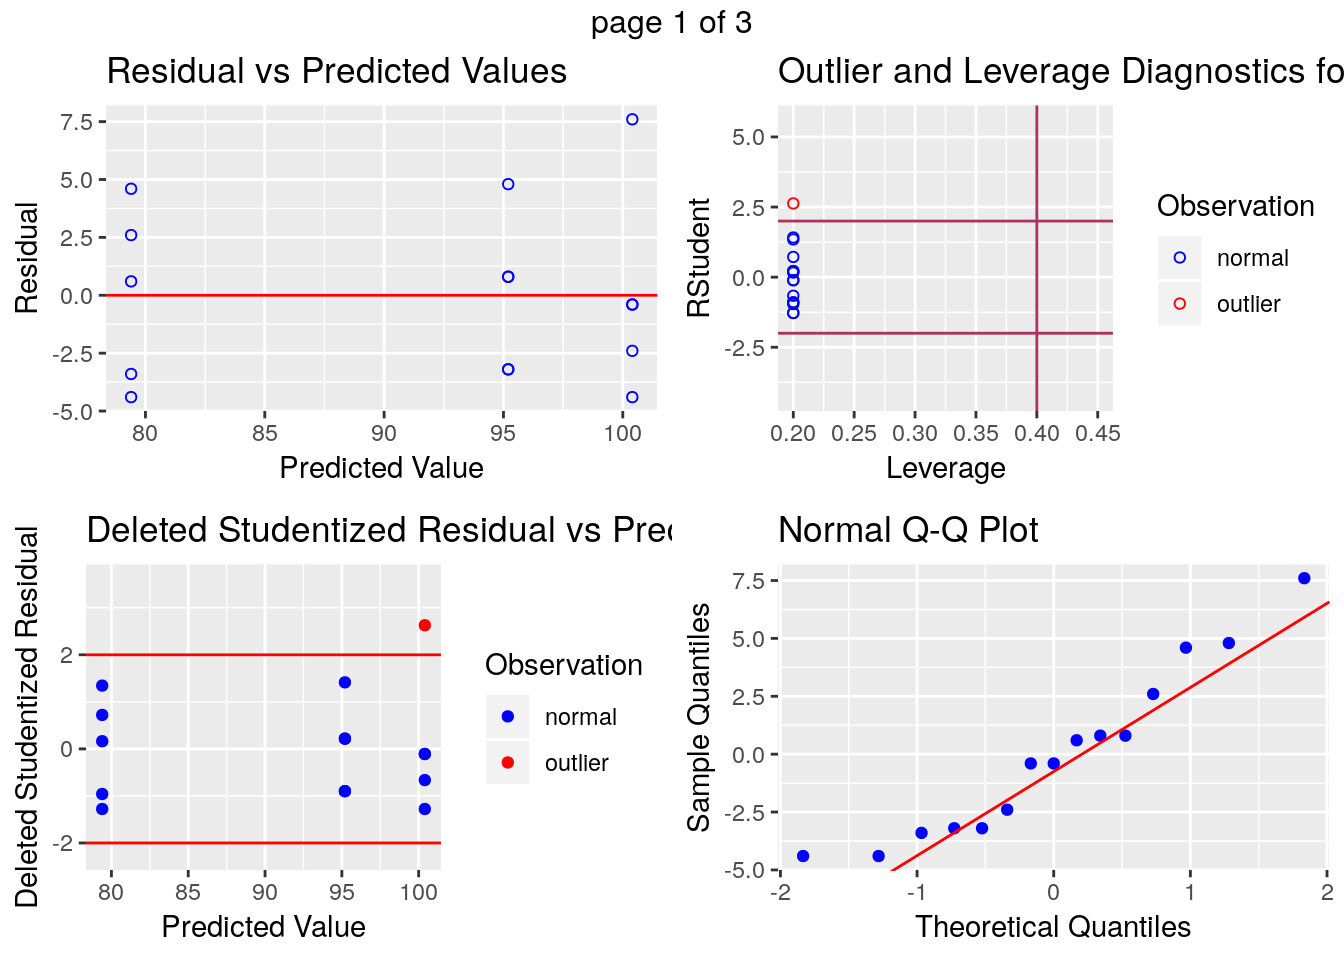
\includegraphics[width=0.25\linewidth]{lab_stat565_files/figure-latex/unnamed-chunk-5-1}
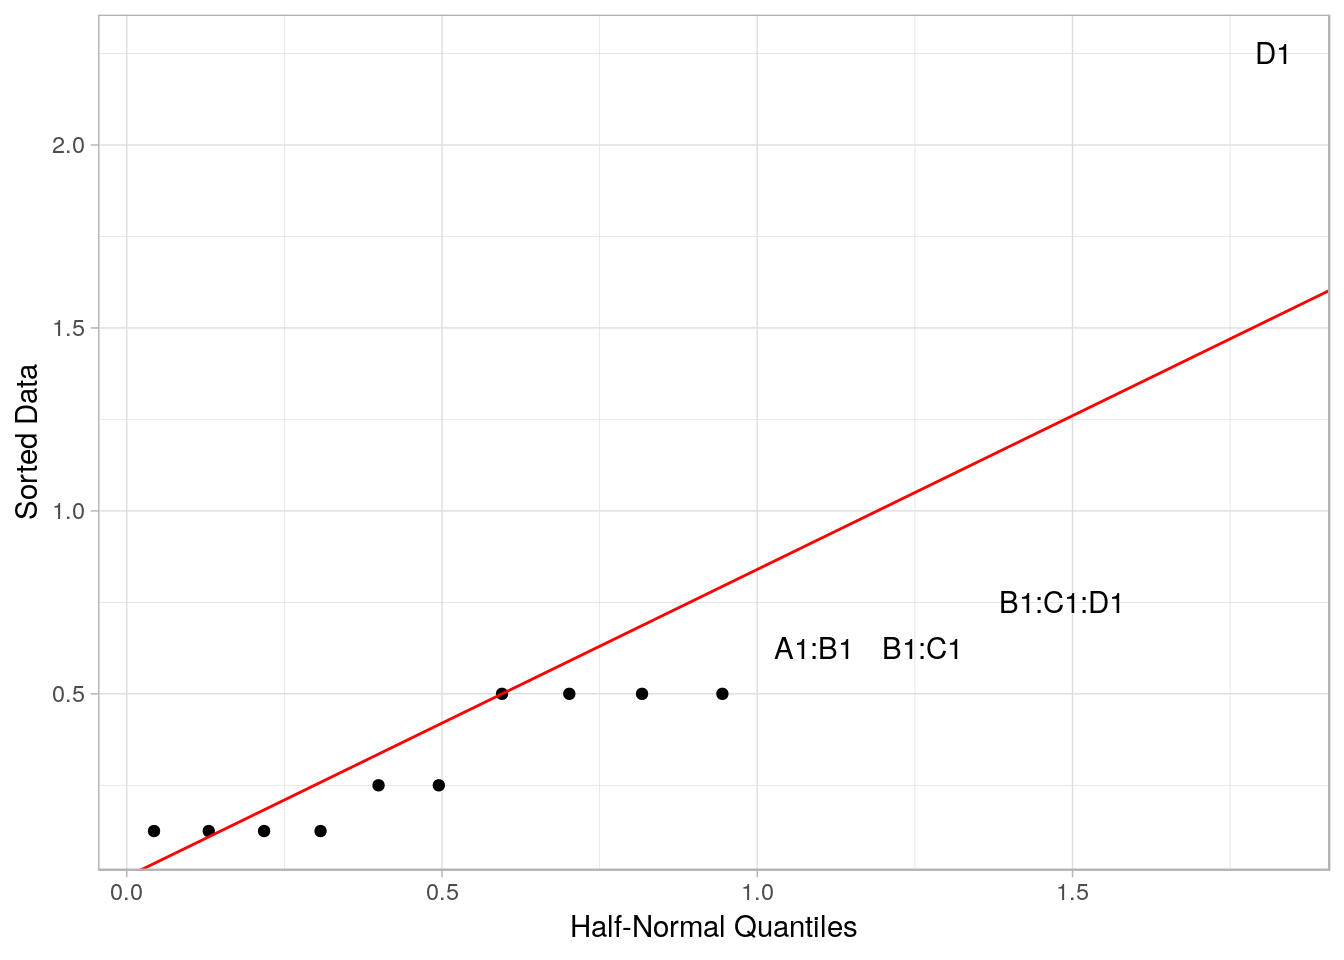
\includegraphics[width=0.25\linewidth]{lab_stat565_files/figure-latex/unnamed-chunk-5-2}
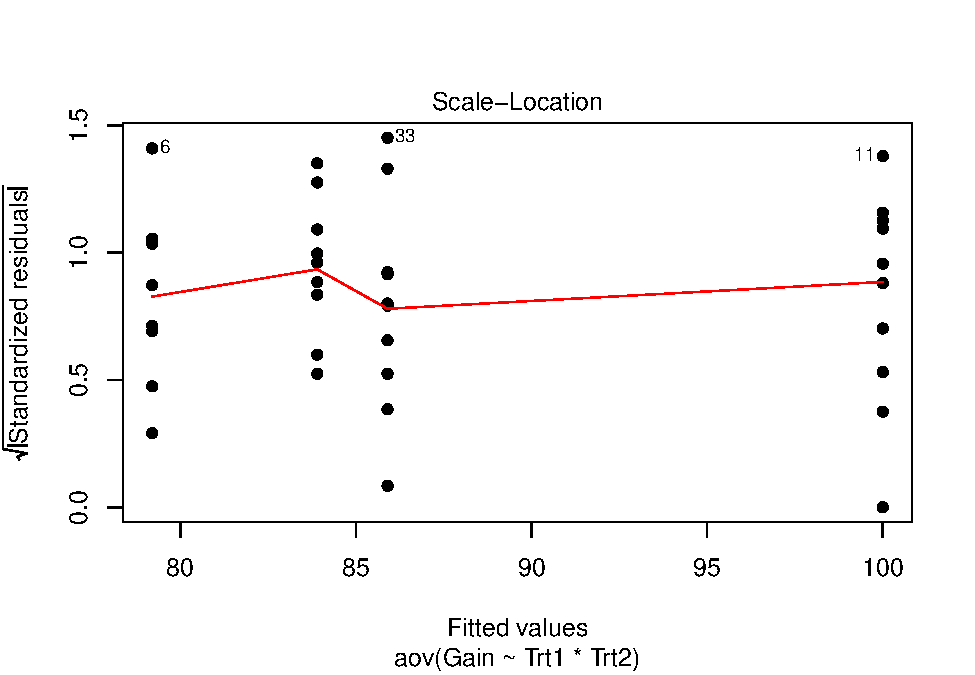
\includegraphics[width=0.25\linewidth]{lab_stat565_files/figure-latex/unnamed-chunk-5-3}
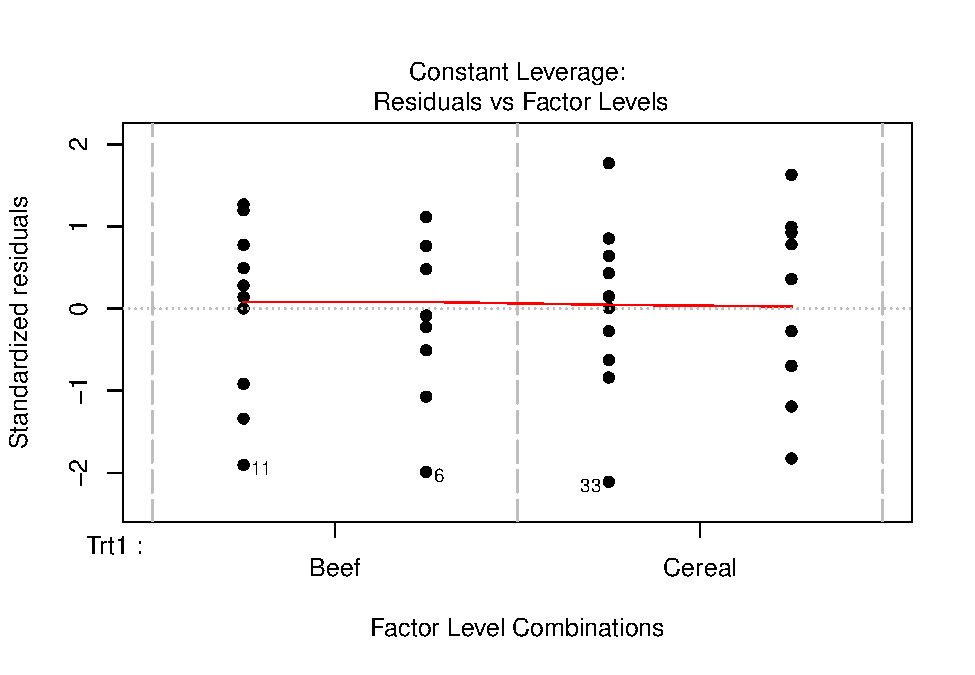
\includegraphics[width=0.25\linewidth]{lab_stat565_files/figure-latex/unnamed-chunk-5-4}

\{(f).
\textcolor[rgb]{0.5,0.5,0.5}{Based on the residual plots, clearly explain whether assumptions in the model are satisfied or violated.}

The plot of studentized residual versus predicted (fitted) value shows
that except few outliers, the residuals are evenly distributed about
zero at each prededict value (zero mean) and vertical deviations of
residuals from zero are about same for each predicted value (constant
variance).

The plots of studentized residual versus factor levels didn't show
obvious violation of zero mean and constant variance.

The QQ plot shows that some data points are not on the line and
flattening at the extremes, which is a litte violation of normality.

(g). \textcolor[rgb]{0.5,0.5,0.5}{Report the code here without output.}

\begin{Shaded}
\begin{Highlighting}[]
\NormalTok{table_protein <-}\StringTok{ }\KeywordTok{read_excel}\NormalTok{(}\StringTok{"Protein.xlsx"}\NormalTok{)}
\KeywordTok{glimpse}\NormalTok{(table_protein)}
\KeywordTok{ggplot}\NormalTok{(}\DataTypeTok{data =}\NormalTok{ table_protein, }\KeywordTok{aes}\NormalTok{(}\DataTypeTok{x =}\NormalTok{ Amount, }\DataTypeTok{y =}\NormalTok{ Gain, }\DataTypeTok{colour =}\NormalTok{ Source, }\DataTypeTok{group =}\NormalTok{ Source)) }\OperatorTok{+}\StringTok{ }
\StringTok{    }\KeywordTok{geom_point}\NormalTok{(}\KeywordTok{aes}\NormalTok{(}\DataTypeTok{shape =}\NormalTok{ Source, }\DataTypeTok{color =}\NormalTok{ Source), }\DataTypeTok{size =} \DecValTok{2}\NormalTok{) }\OperatorTok{+}\StringTok{ }\KeywordTok{labs}\NormalTok{(}\DataTypeTok{y =} \StringTok{"Weight Gained"}\NormalTok{, }
    \DataTypeTok{x =} \StringTok{"Amount of table_protein"}\NormalTok{, }\DataTypeTok{color =} \StringTok{"Source of table_protein"}\NormalTok{, }\DataTypeTok{shape =} \StringTok{"Source of table_protein"}\NormalTok{)}
\CommentTok{# Plots the Mean and 1SD error bars for each treatment group #}
\KeywordTok{ggplot}\NormalTok{(}\DataTypeTok{data =}\NormalTok{ table_protein, }\KeywordTok{aes}\NormalTok{(}\DataTypeTok{x =}\NormalTok{ Amount, }\DataTypeTok{y =}\NormalTok{ Gain, }\DataTypeTok{colour =}\NormalTok{ Source, }\DataTypeTok{shape =}\NormalTok{ Source, }
    \DataTypeTok{group =}\NormalTok{ Source)) }\OperatorTok{+}\StringTok{ }\KeywordTok{stat_summary}\NormalTok{() }\OperatorTok{+}\StringTok{ }\KeywordTok{labs}\NormalTok{(}\DataTypeTok{y =} \StringTok{"Weight Gained"}\NormalTok{, }\DataTypeTok{x =} \StringTok{"Amount of table_protein"}\NormalTok{, }
    \DataTypeTok{color =} \StringTok{"Source"}\NormalTok{, }\DataTypeTok{shape =} \StringTok{"Source"}\NormalTok{)}
\CommentTok{# Install and load ggpubr package before using ggline function #}
\KeywordTok{ggline}\NormalTok{(}\DataTypeTok{data =}\NormalTok{ table_protein, }\DataTypeTok{x =} \StringTok{"Amount"}\NormalTok{, }\DataTypeTok{y =} \StringTok{"Gain"}\NormalTok{, }\DataTypeTok{add =} \KeywordTok{c}\NormalTok{(}\StringTok{"mean"}\NormalTok{, }\StringTok{"jitter"}\NormalTok{), }
    \DataTypeTok{shape =} \StringTok{"Source"}\NormalTok{, }\DataTypeTok{color =} \StringTok{"Source"}\NormalTok{, }\DataTypeTok{linetype =} \StringTok{"Source"}\NormalTok{, }\DataTypeTok{ylab =} \StringTok{"Weight Gained"}\NormalTok{, }
    \DataTypeTok{xlab =} \StringTok{"Amount of table_protein"}\NormalTok{)}
\CommentTok{# Load mosaic package before using favstats function#}
\KeywordTok{favstats}\NormalTok{(Gain }\OperatorTok{~}\StringTok{ }\NormalTok{Source, }\DataTypeTok{data =}\NormalTok{ table_protein)}
\KeywordTok{favstats}\NormalTok{(Gain }\OperatorTok{~}\StringTok{ }\NormalTok{Amount, }\DataTypeTok{data =}\NormalTok{ table_protein)}
\KeywordTok{favstats}\NormalTok{(Gain }\OperatorTok{~}\StringTok{ }\NormalTok{Source }\OperatorTok{|}\StringTok{ }\NormalTok{Amount, }\DataTypeTok{data =}\NormalTok{ table_protein)}
\KeywordTok{favstats}\NormalTok{(Gain }\OperatorTok{~}\StringTok{ }\NormalTok{Source }\OperatorTok{+}\StringTok{ }\NormalTok{Amount, }\DataTypeTok{data =}\NormalTok{ table_protein)}

\NormalTok{table_protein}\OperatorTok{$}\NormalTok{Trt1 =}\StringTok{ }\KeywordTok{as.factor}\NormalTok{(table_protein}\OperatorTok{$}\NormalTok{Source)}
\NormalTok{table_protein}\OperatorTok{$}\NormalTok{Trt2 =}\StringTok{ }\KeywordTok{as.factor}\NormalTok{(table_protein}\OperatorTok{$}\NormalTok{Amount)}
\NormalTok{model_protein <-}\StringTok{ }\KeywordTok{aov}\NormalTok{(Gain }\OperatorTok{~}\StringTok{ }\NormalTok{Trt1 }\OperatorTok{*}\StringTok{ }\NormalTok{Trt2, }\DataTypeTok{data =}\NormalTok{ table_protein)}
\KeywordTok{summary}\NormalTok{(model_protein)}
\KeywordTok{pander}\NormalTok{(}\KeywordTok{summary}\NormalTok{(model_protein))}
\KeywordTok{sum}\NormalTok{((table_protein}\OperatorTok{$}\NormalTok{Gain }\OperatorTok{-}\StringTok{ }\KeywordTok{mean}\NormalTok{(table_protein}\OperatorTok{$}\NormalTok{Gain))}\OperatorTok{^}\DecValTok{2}\NormalTok{)}
\KeywordTok{plot}\NormalTok{(model_protein, }\DataTypeTok{pch =} \DecValTok{16}\NormalTok{)}
\CommentTok{# Pairwise comparisons using t tests with pooled Standard Deviation # The}
\CommentTok{# output gives a matrix of p values for each pair of treatments #}
\KeywordTok{pairwise.t.test}\NormalTok{(table_protein}\OperatorTok{$}\NormalTok{Gain, table_protein}\OperatorTok{$}\NormalTok{Trt2, }\DataTypeTok{p.adj =} \StringTok{"none"}\NormalTok{)}
\CommentTok{# Pairwise comparisons using t tests with pooled Standard Deviation and}
\CommentTok{# Bonferroni adjustment # The output gives a matrix of p values for each}
\CommentTok{# pair of treatments #}
\KeywordTok{pairwise.t.test}\NormalTok{(table_protein}\OperatorTok{$}\NormalTok{Gain, table_protein}\OperatorTok{$}\NormalTok{Trt2, }\DataTypeTok{p.adj =} \StringTok{"bonf"}\NormalTok{)}
\CommentTok{# Install and load the agricolae package before running the LSD.test}
\CommentTok{# function below # p.adj option in the LSD.test function can be used to}
\CommentTok{# apply different adjustments to control error rates#}
\KeywordTok{plot}\NormalTok{(}\KeywordTok{LSD.test}\NormalTok{(model_protein, }\DataTypeTok{trt =} \StringTok{"Trt2"}\NormalTok{, }\DataTypeTok{alpha =} \FloatTok{0.05}\NormalTok{))}
\NormalTok{(}\KeywordTok{LSD.test}\NormalTok{(model_protein, }\DataTypeTok{trt =} \StringTok{"Trt2"}\NormalTok{, }\DataTypeTok{alpha =} \FloatTok{0.05}\NormalTok{))}
\KeywordTok{pander}\NormalTok{(}\KeywordTok{TukeyHSD}\NormalTok{(model_protein, }\DataTypeTok{conf.level =} \FloatTok{0.95}\NormalTok{)[}\DecValTok{3}\NormalTok{])}
\KeywordTok{pander}\NormalTok{(}\KeywordTok{ScheffeTest}\NormalTok{(model_protein, }\DataTypeTok{conf.level =} \FloatTok{0.95}\NormalTok{)[}\DecValTok{3}\NormalTok{])}
\end{Highlighting}
\end{Shaded}


\end{document}
